\subsection{Software} \label{sec:Software}
\textit{pro} Die Software des Planting Robots ist in der Programmiersprache C geschrieben und läuft auf dem ARM Cortex M0+ Mikrocontroller von NXP welcher auf dem FRDM-Board KL25Z bestückt ist. Als Betriebssystem dient das Real Time OS FreeRTOS. Vorteile von FreeRTOS gegenüber anderen C Betriebssystemen sind:

\begin{itemize}
	\item Seine geringen Ressourcenanforderungen an RAM, ROM und CPU Leistung. 
	\item FreeRTOS ist weit verbreitet und wird an der HSLU in diversen Softwareprojekten verwendet.
	\item Es ist absolut kostenfrei, auch für kommerzielle Anwendungen.
	\item FreeRTOS ist einfach in der Anwendung, eignet sich jedoch auch für grössere Projekte.
\end{itemize}

In den folgenden Unterkapiteln werden die wichtigsten Softwarekomponenten des Planting Robots beschrieben und erklärt. Die Titel der Unterkapitel korrespondieren dabei mit den Namen der .c Files des Codes im Anhang.

\subsubsection{FSM}
Der Planting Robot wird durch einen endlichen Zustandsautomaten FSM gesteuert. Die Zustände oder States die FSM sind in Abb. \ref{fig:FSM} illustriert. Ein State Wechsel wird entweder durch eine User Eingabe übe das HMI, eine Topferkennung durch den IR-Sensor oder durch fertigstellen eines States ausgeführt. Im folgenden Abschnitt werden die verschiedenen States sowie State-Wechsel erklärt:

\begin{figure}[H]
	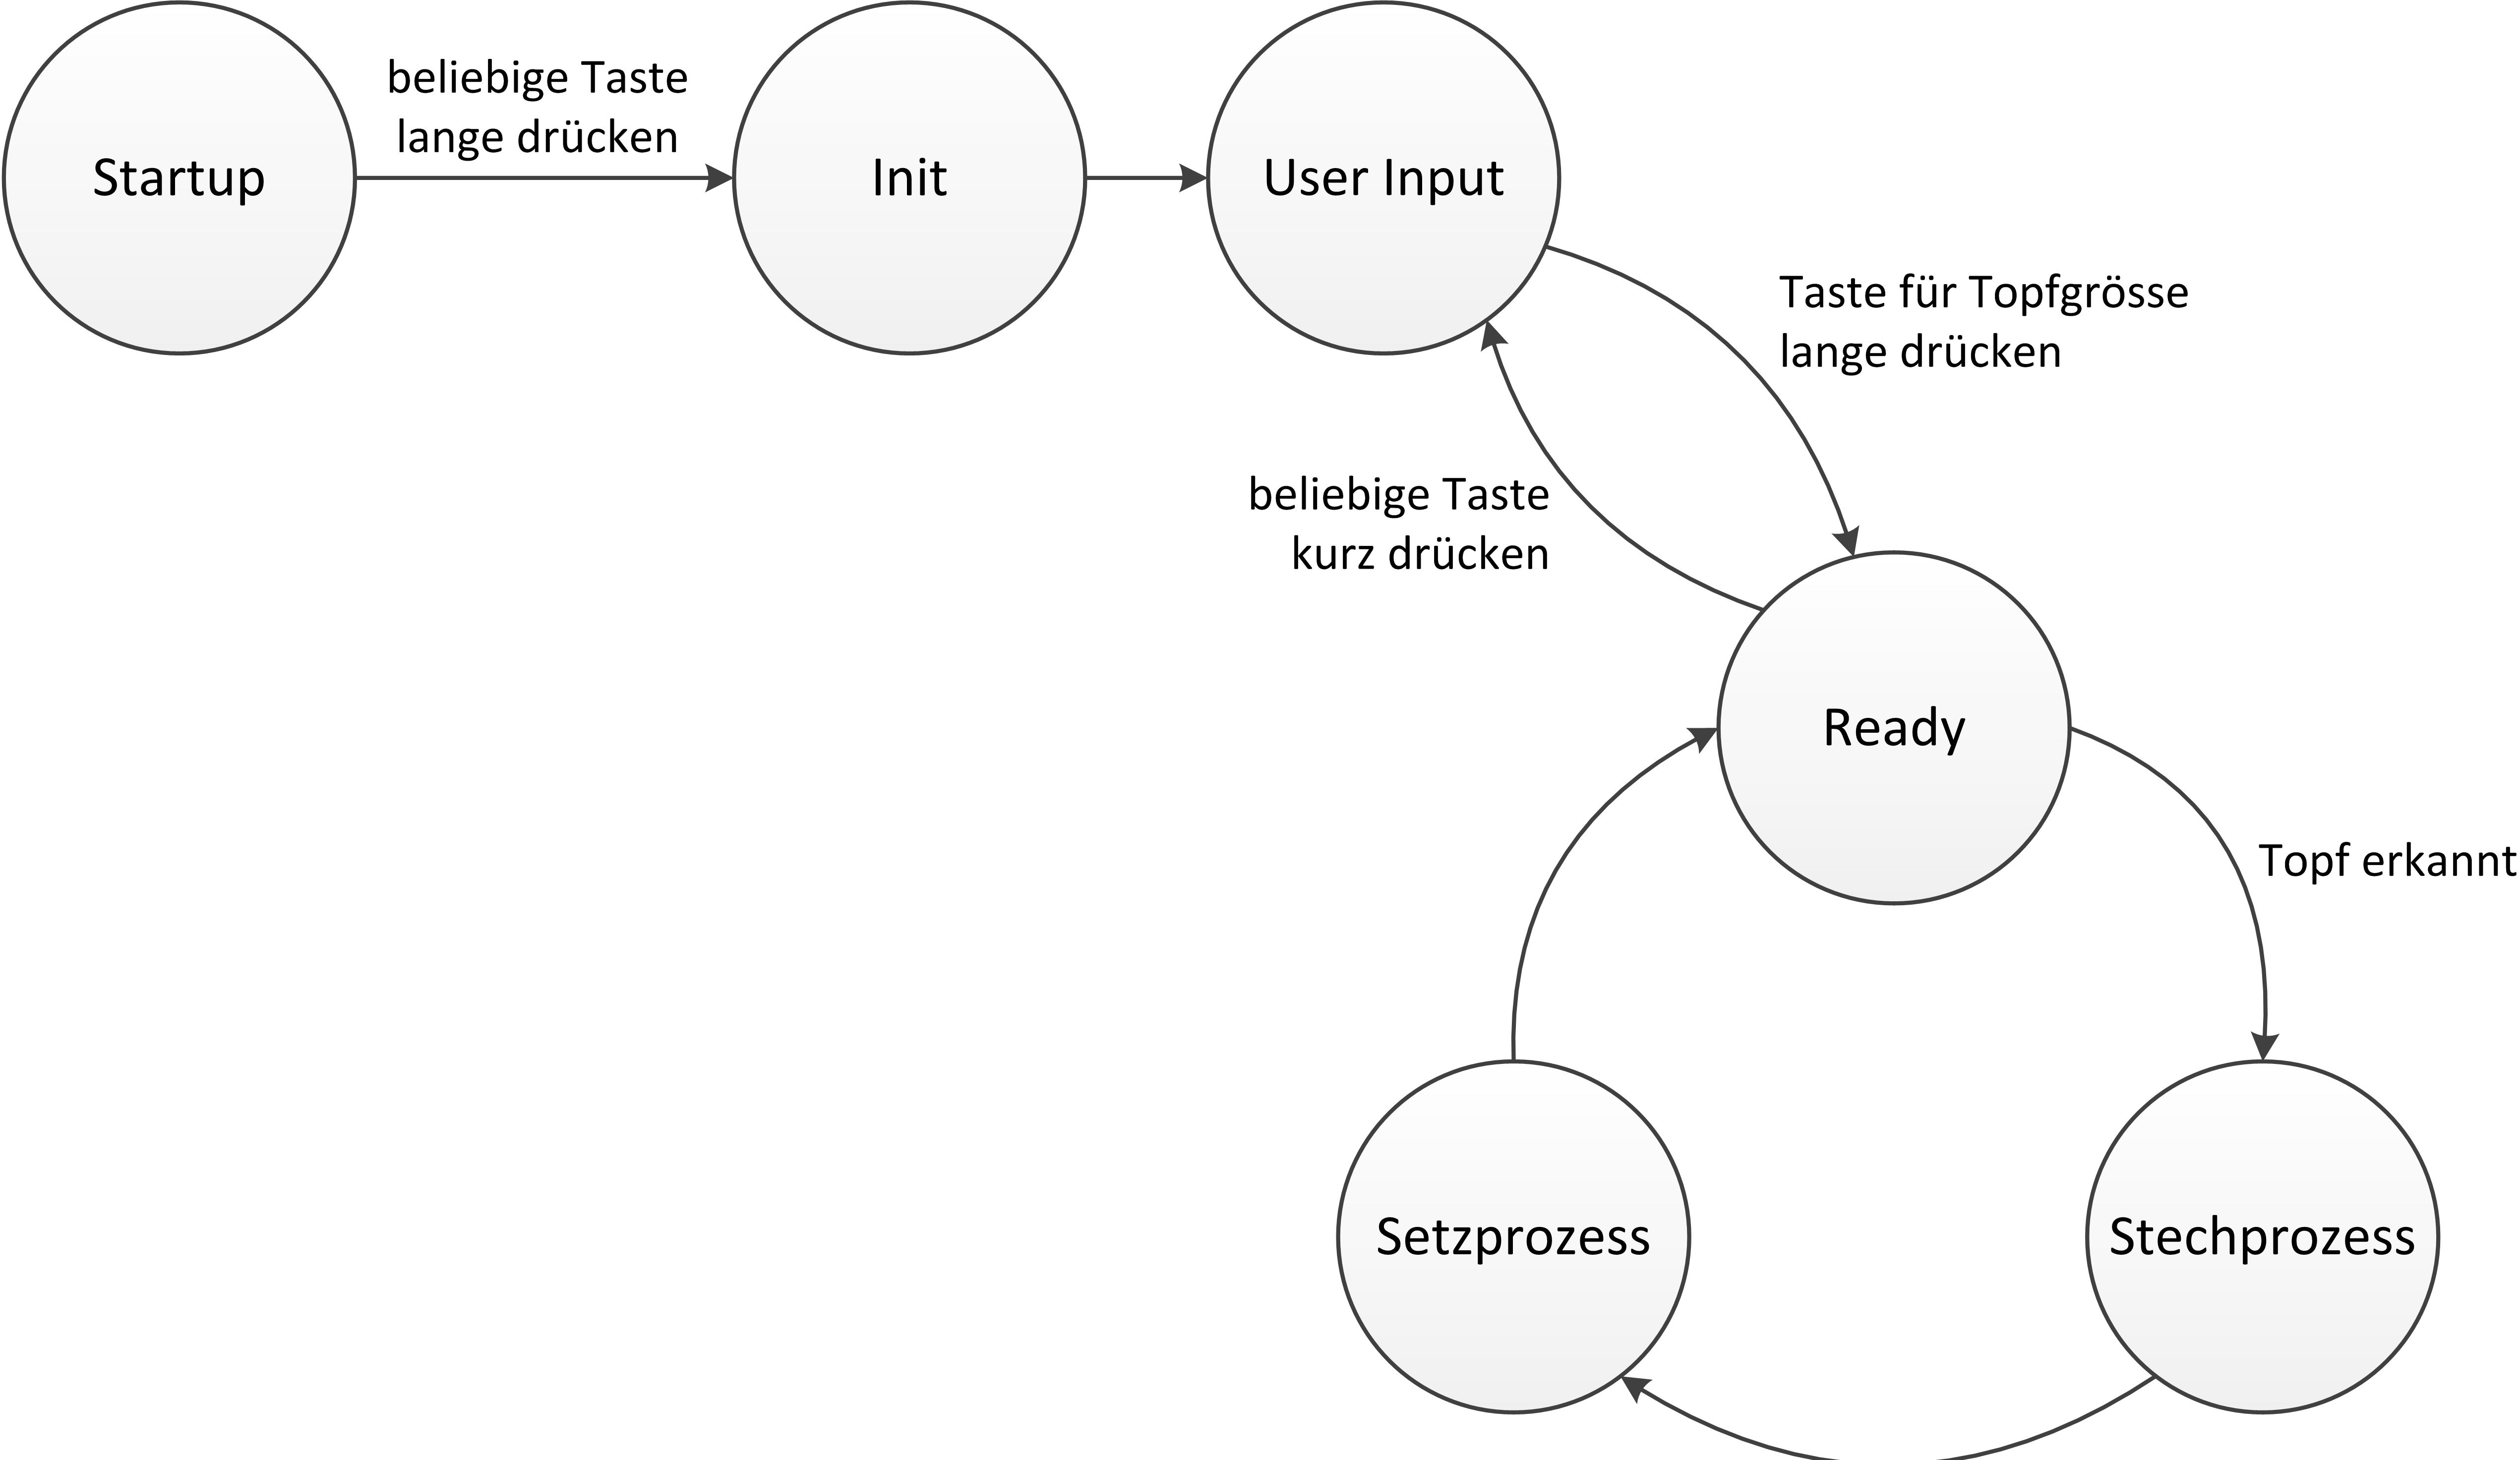
\includegraphics[width=0.9\textwidth]{Illustrationen/6-Umsetzung/FSM_B&W_breit.png}
	\caption{Software, FSM}
	\label{fig:FSM}
\end{figure}

\textbf{Startup:} Wenn die Speisung zum uC eingeschaltet wird, begibt sich die Software in den sicheren Zustand $"$Startup$"$. In diesem State sind sämtliche Aktoren stromlos. Alle LEDs des HMIs pulsieren synchron. Wird ein beliebiger Taster des HMIs länger als eine halbe Sekunde gedrückt wechselt die Software in den $"$Init$"$ State.\\
\newline
\textbf{Init:} In diesem State werden die Motoren für die Vereinzelung, die Verstellmechanik und die Setzeinheit initialisiert. Da die Motoren über Drehencoder und nicht über absolute Positionsencoder verfügen, müssen diese zuerst in ihre Ausgangsposition gebracht werden. Der Initialisierungsprozess zu den jeweiligen Motoren wird in den Kapiteln \ref{sec:Vereinzelung}, \ref{sec:Setzeinheit} und \ref{verstellmechanik} erklärt. Während der Initialisierung blinken die HMI LEDs des jeweiligen Prozesses. Nach Abschluss der Initialisierung wechselt die State Machine in den $"$User Input$"$ State.\\
\newline
\textbf{User Input:} Dieser State dient zur Konfiguration des Planting Robots. Der Operator kann hier die Topfgrösse des aktuellen Batches und die Setztiefe der Nemacaps über das HMI einstellen. Ausserdem kann der Planting Robot in diesem State manuell über die Tasten $"$manuelle Steuerung$"$ bedient werden. Mehr zur manuellen Steuerung ist im Kapitel \ref{sec:HMI} nachzulesen. Um die Konfiguration zu speichern und den Planting Robot in Betrieb zu setzen muss der Taster für die gewünschte Topfgrösse lange gedrückt werden.\\
\newline
\textbf{Ready:} Der Planting Robot befindet sich im regulären Betriebsmodus. Sobald ein Topf erkannt wird, verrichtet der Planting Robot seine Arbeit indem er den Stechprozess und anschliessend den Setzprozess ausführt. Um den Planting Robot zu stoppen, kann ein beliebiger Taster gedrückt werden. Der Planting Robot wechselt dann zurück in den $"$User Input$"$ State.\\
\newline
\textbf{Stechprozess:} Dieser Prozess wird durchlaufen sobald ein Topf erkannt wurde. Dabei wird mit dem Spindelantrieb eine Hubbewegung ausgeführt bei welcher der Stechdorn in die Erde gedrückt und wieder angehoben wird.\\
\newline
\textbf{Setzprozess:} Sobald der Stechprozess beendet ist wird der Setzprozess ausgeführt. Dabei wird die Vereinzlung angetrieben, sodass NemaCaps vom Schüttgutlager in die Topferde befördert wird. Nach beenden des Setzprozesses geht die FSM wieder in den $"$Ready$"$ State.

\subsubsection{HMI Driver}

\subsubsection{LED Driver}

\subsubsection{ION Motion Driver}

\subsubsection{IR Sensor Driver}

\subsubsection{Trinamic Motion Driver}